\documentclass{article}%book,report,letter

\usepackage{ctex}
\usepackage{fontspec}
%\usepackage{color}
%\usepackage{graphicx} %use graph format
%\usepackage{subfigure}
%\usepackage{epstopdf} %eps图片
\usepackage{amsmath}  %字体加粗
%\usepackage{math}
\usepackage{amsthm}
\usepackage{amssymb} %因为所以符号
%\usepackage{caption}
%\captionsetup[table]{labelsep=space}
\usepackage{float}%图片位置

%自定义命令
\newcommand*{\myTestTimes}{1\xspace}
%\typein[\myTestTimes]{这是第几次测试?}
\newcommand*{\myName}{桑明达\xspace}
\newcommand*{\myNumber}{15300180062\xspace}
\newcommand*{\myHomeworkNumber}{第十二周作业\xspace}
\newcommand*{\myArticleName}{微分方程数值解法\xspace}

\newcommand*{\myseries}[2][n]{\ensuremath{#2_1,#2_2,\dots,#2_{#1}}}


%制作页眉页脚
\usepackage{fancyhdr}
\pagestyle{fancy}
\lhead{\myHomeworkNumber}
\chead{\myArticleName}
\rhead{\myName \myNumber}
\lfoot{}
\cfoot{\thepage}
\rfoot{}
\renewcommand{\headrulewidth}{0.4pt}
\renewcommand{\footrulewidth}{0.4pt}

%标题
\title{\heiti \myArticleName \\ [2ex] \begin{large} \myHomeworkNumber \end{large}}
\author{\kaishu \myName \myNumber}
\date{\today}

% 正文区
\begin{document}
\maketitle

%\newpage

\section{P195 式4.2.16 Richardson}

\begin{proof}
	\begin{align*}
		R^n_i = & \frac{u_i^{n+1}-u_i^{n-1}}{2 \tau }- a \Delta _h u_i^n - \left ( u_t(t_n,x_i)-au_{xx}(t_n,x_i) \right )  \\
			= & \left (\frac{u_i^{n+1}-u_i^{n-1}}{2 \tau } - u_t(t_n,x_i)  \right )  - \left (a \Delta _h u_i^n -au_{xx}(t_n,x_i)  \right ) \\
			= & \frac{\tau^2}{6}\frac{\partial ^3 u}{\partial t^3}(t_n,x_i)+ O(\tau^4)-\frac{ah^2}{12}\frac{\partial ^4 u}{\partial t^4}(t_n,x_i)+O(h^4) \\
	\end{align*}
\end{proof}

\section{P195 1 抛物线方程}

\begin{proof}
\par
(1)解析解未求出,时间和空间都100等分为101点,得到计算结果如图

\begin{figure}[H]
	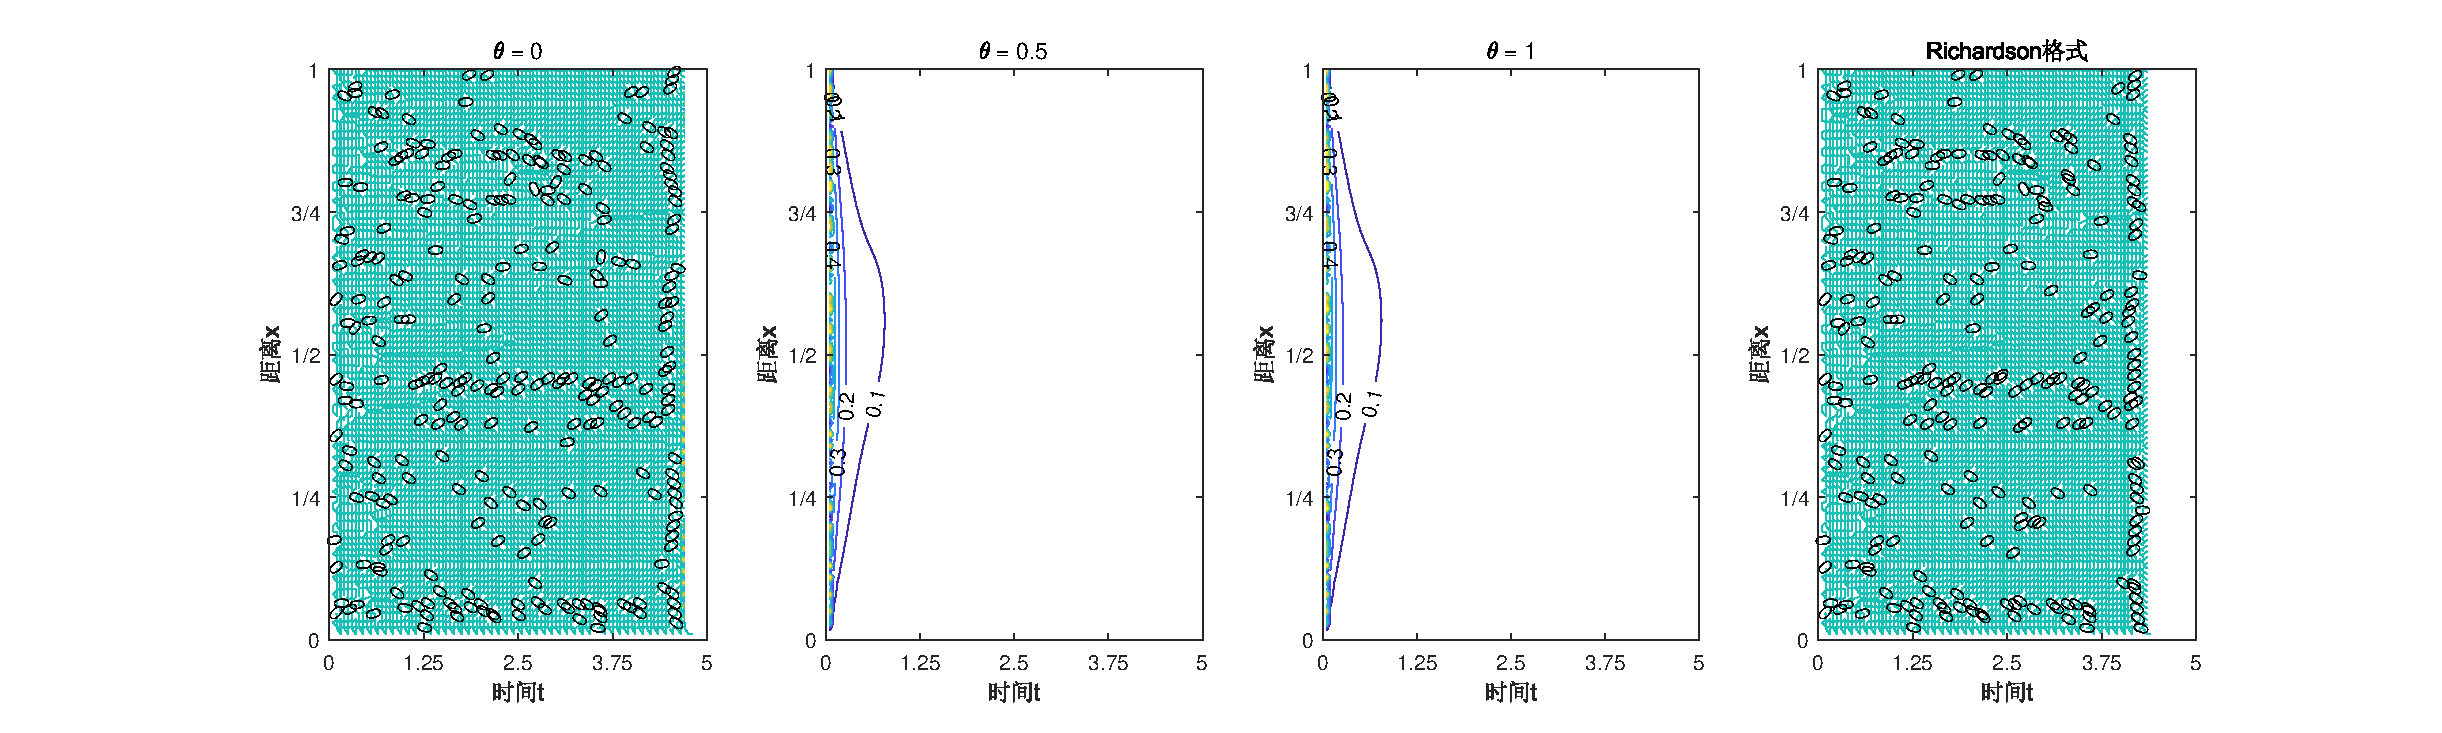
\includegraphics[width=1\linewidth]{week12_1_1.eps}
	%\caption{三点差分格式离散求解}
	\label{Fig:1.1}
\end{figure}


可以看出,$\theta$ = 0.5或1时,格式结果较好,其中$\theta$ = 1时,收敛到0。

(2)解析解为$$ u(t,x)=\frac{1-e^{-\pi^2t}}{\pi^2}\sin \pi x + \frac{1-e^{-4\pi^2t}}{4\pi^2}\sin 2\pi x $$

时间和空间都100等分为101点,得到计算结果如图

\begin{figure}[H]
	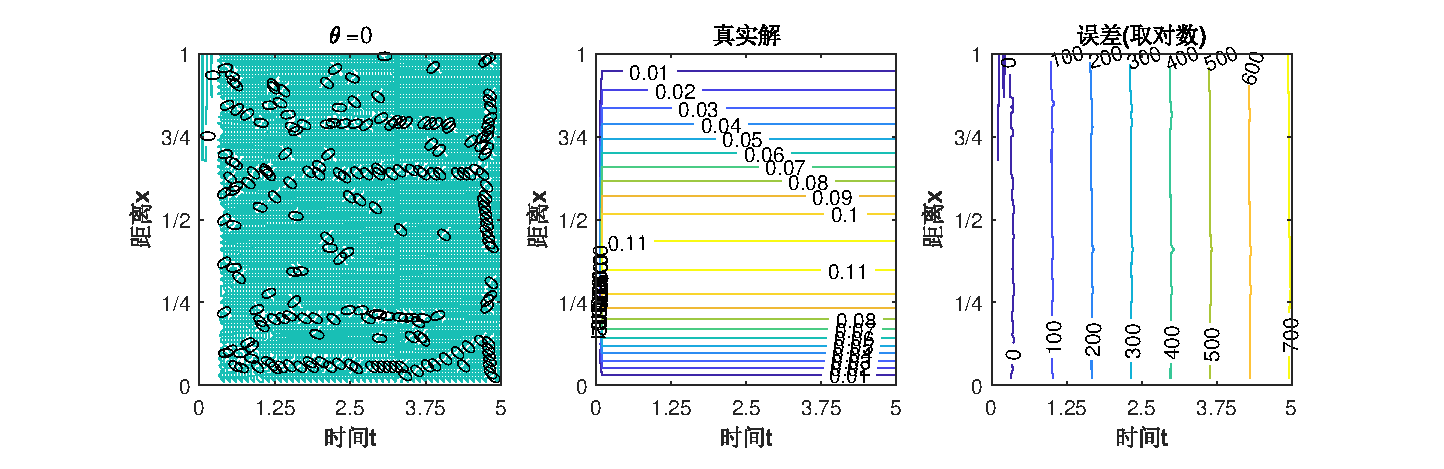
\includegraphics[width=1\linewidth]{week12_2_1.eps}
	%\caption{三点差分格式离散求解}
	\label{Fig:2.1}
\end{figure}

\begin{figure}[H]
	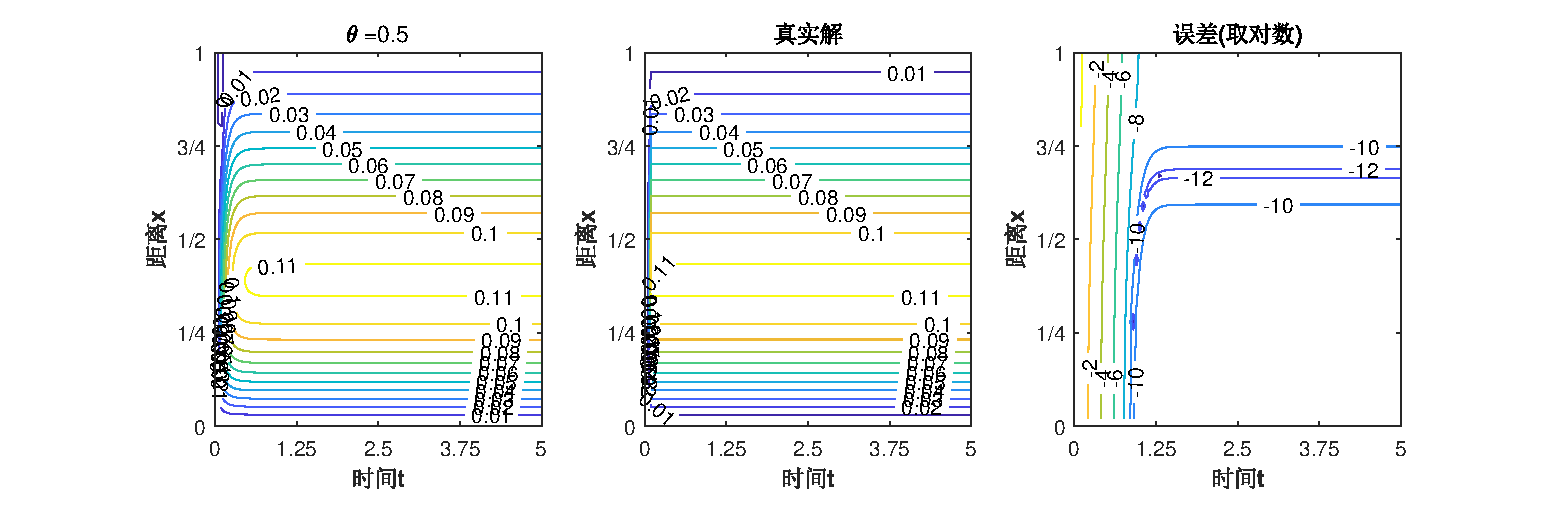
\includegraphics[width=1\linewidth]{week12_2_2.eps}
	%\caption{三点差分格式离散求解}
	\label{Fig:2.2}
\end{figure}

\begin{figure}[H]
	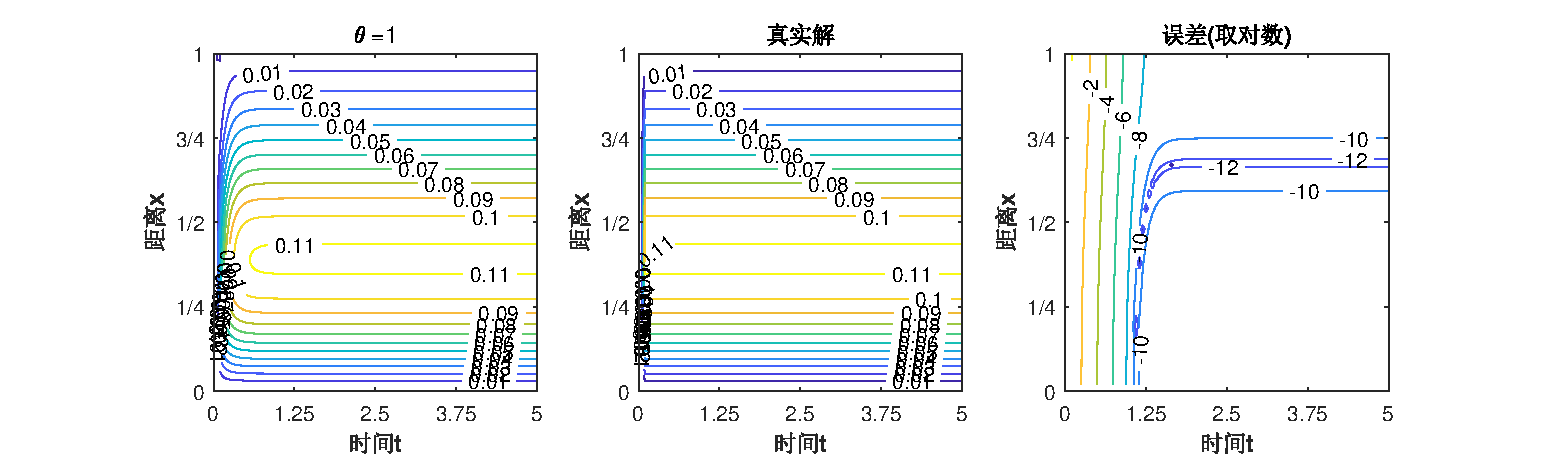
\includegraphics[width=1\linewidth]{week12_2_3.eps}
	%\caption{三点差分格式离散求解}
	\label{Fig:2.3}
\end{figure}

\begin{figure}[H]
	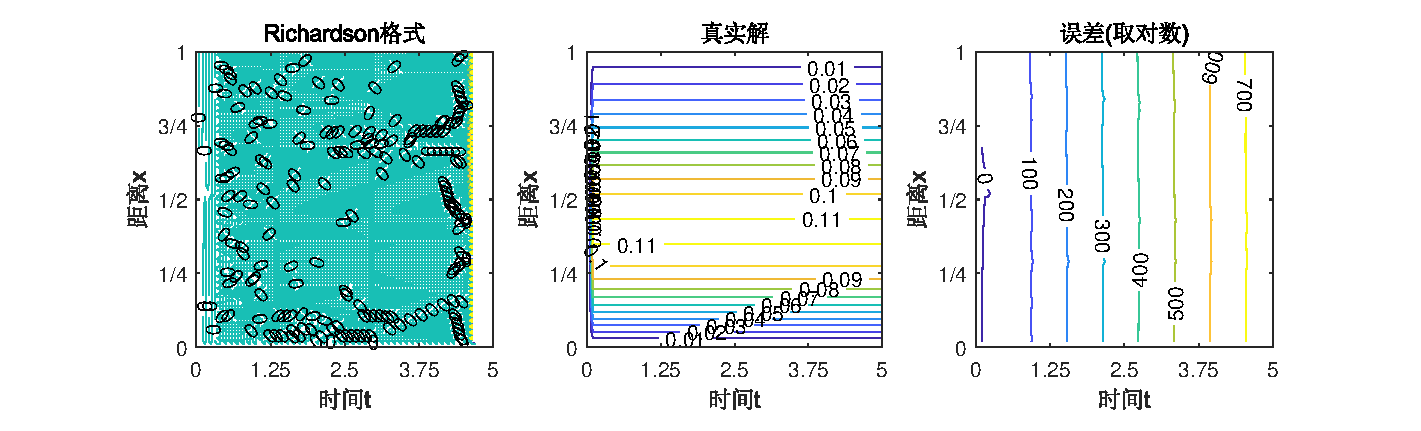
\includegraphics[width=1\linewidth]{week12_2_4.eps}
	%\caption{三点差分格式离散求解}
	\label{Fig:2.4}
\end{figure}

可以看出,$\theta$ = 0.5或1时,格式结果较好,误差很小,当$t\rightarrow \infty $时,得到的边值问题的解一致。
\end{proof}

\end{document}
